
\section*{Problema P8.33}

\renewcommand*\thesection{8.33}
\numberwithin{equation}{section}

\begin{center}
    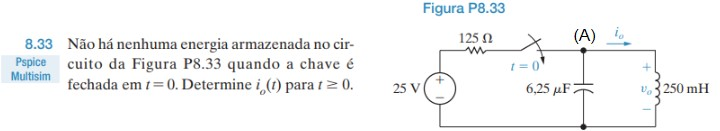
\includegraphics[scale=1.0]{P8.33.jpg}
\end{center}

Aplicamos análise nodal no nó essencial (A) em $t>0$.

\[ i_R + i_C + i_L = 0  \]

\[ \frac{v_o - 25}{R} + C\diff{v_o}{t} + i_o = 0  \]

Note que 

\[ v_0 = L\diff{i_o}{t}  \]

Assim, a equação nodal se torna 

\[ \frac{L\diff{i_o}{t} - 25}{R} + C\diff{L\diff{i_o}{t}}{t} + i_o = 0  \]

\[ \frac{L\diff{i_o}{t} - 25}{R} + C\diff{\left(L\diff{i_o}{t}\right)}{t} + i_o = 0  \]

\[ \diff[2]{i_o}{t} + \frac{1}{RC} \diff{i_o}{t} + \frac{i_o}{LC} + \frac{25}{RLC} = 0  \]

Substituindo com os valores do enunciado, temos  

\[ \diff[2]{i_o}{t} + 1280\diff{i_o}{t} + 640000i_o + 128000 = 0  \]

Observação: tentei resolver a EDO acima com o método que usei nas questões anteriores:  admitindo solução na forma
$i_o(t) = Ae^{-st}$ e achando os coeficientes através das condições iniciais do circuito.
Contudo, não consegui identificar as condições iniciais e não achei a resposta correta. Tentei resolver
pelo método dado em sala da aula, mas não sei Transformada de Laplace muito bem e as fotos que tirei do quadro ficaram ruins. 
Assim, coloco diretamente a solução dada em sala de aula dessa questão via Laplace.

\[ \boxed{i_o(t) = 0.2u(t) - 0.2e^{-640t}\cos(480t) - \frac{4}{15}e^{-640t}\sin(480t) \un{A} \, , \, t \geq 0} \]

Onde $u(t)$ é a função degrau unitário.


